\documentclass[11pt]{article}
\usepackage{geometry}                % See geometry.pdf to learn the layout options. There are lots.
\geometry{letterpaper}                   % ... or a4paper or a5paper or ... 
%\geometry{landscape}                % Activate for for rotated page geometry
%\usepackage[parfill]{parskip}    % Activate to begin paragraphs with an empty line rather than an indent
\usepackage{graphicx}
\usepackage{amssymb}
\usepackage{epstopdf}

\usepackage{amsmath}
\usepackage{amssymb}

\usepackage{placeins}
\usepackage{harpoon}

\usepackage{longtable}

\usepackage[square,numbers]{natbib}

\DeclareGraphicsRule{.tif}{png}{.png}{`convert #1 `dirname #1`/`basename #1 .tif`.png}

%\input{Macros.tex}
\title{HPS Note:  Time Dependent Ecal callibrations}
\author{Sebouh Paul}
\date{}                                           % Activate to display a given date or no date

\begin{document}
\maketitle
\section{Introduction}
This investigation began when I found that the positions of the full energy electron (FEE) and two cluster energy sum (2CES) peaks, as measured by the Ecal in the 2016 dataset, did not remain constant as a function of time.   This prompted me to investigate further, and found that this phenomenon also occurred in the 2015 dataset as well.  This sort of behavior is not unique to HPS; such behavior has been found in the CLAS experiment as well, which uses the same type of electromagnetic calorimeter as well.  To remedy this issue, I have created a list of parameterizations to use for each run, which we can use to scale uniformly scale every cluster read out in the Ecal.  

\section{Outline of procedure}
First I created histograms of the single cluster energies, and 2 cluster energy sums (with certain cuts to isolate the peaks, explained in detail in the next section) for the first file in each of the ``golden runs" in the 2015 and 2016 datasets.  For the 2015 golden run selection, I used the ones that Sho and Holly had posted in the 2015 run spreadsheet.  For the 2016 data, I used my own list of golden runs (which i describe in one of my other analysis notes).  Next, I fitted these histograms to a crystal ball function to find the peak energy for the 2CES and the FEE peak.  Then, I plotted these out as a function of run number and of the starting time of the run.  Finally, i determined a parameterization of the FEE peak position as a function of time.   

To test this parameterization for legitimacy, I plotted the 2CES peak position multiplied by the correction factor obtained by dividing the beam energy by the FEE peak position.  If this corrected peak position remains approximately constant after making these corrections, then this supports my hypothesis that the cluster energies were only off by a simple scaling factor.  

\section{Cuts when making histograms}

For the FEE's, the event must be single1 trigger; the cluster must have at least 3 hits in it, is not seeded on an edge crystal, and that it is matched to a track with at least 90\% of the beam energy (the track cluster matching criterion is to limit the amount of background under the peak and the size of the tail)

For the 2CES histogram, I require that the event be pair1 trigger, and that neither cluster's energy is more than 80\% of the beam energy, the two clusters be on opposite halves of the Ecal, and that neither of them are seeded on an edge crystal.   

\section{Details of Histogram Fitting}
The histograms are fit to a crystal ball function, which has a gaussian core and a power-law tail on the left-hand side.   The formula for a crystal ball function is:

\begin{equation}
N*\begin{cases}
\exp{\frac{-x^2}{2\sigma}},  \frac{x}{\sigma} \ge \alpha\\
A\left(B-\frac{x}{\alpha\sigma}\right)^{-n}, \frac{x}{\sigma} \le \alpha
\end{cases}
\label{eq:crystalball}
\end{equation}

where B and A are defined in terms of $n$, $\alpha$ such that the function and its derivatives are both continuous.

To make the fitting method more consistent between runs, I fixed the value for the parameter $n$ to be 4.5.    I choose to define the limits of the range of fitting relative to the position of the tallest bin, and I have tabulated the choices I used for these parameters in Table \ref{tab:fit_range_limits}.  Figures \ref{fig:one2016_fit_example} through \ref{fig:two2015_fit_example} show examples of these fits.  


\begin{table}[htp]
\caption{Limits of the fit range, relative to the position of the tallest bin in the histogram.  All units in GeV.}
\begin{center}
\begin{tabular}{|c|c|l|l|}
\hline
type & beam energy & fit range min & fit range max \\
\hline
FEE & 1.05 & -.07 & .1 \\
2CES & 1.05 & -.07 & .1 \\ 
FEE & 2.3 & -.2 & .25 \\
2CES & 2.3 & -.2 & .2 \\

\hline
\end{tabular}
\end{center}
\label{tab:fit_range_limits}
\end{table}%

\begin{figure}[htbp] 
\begin{center}
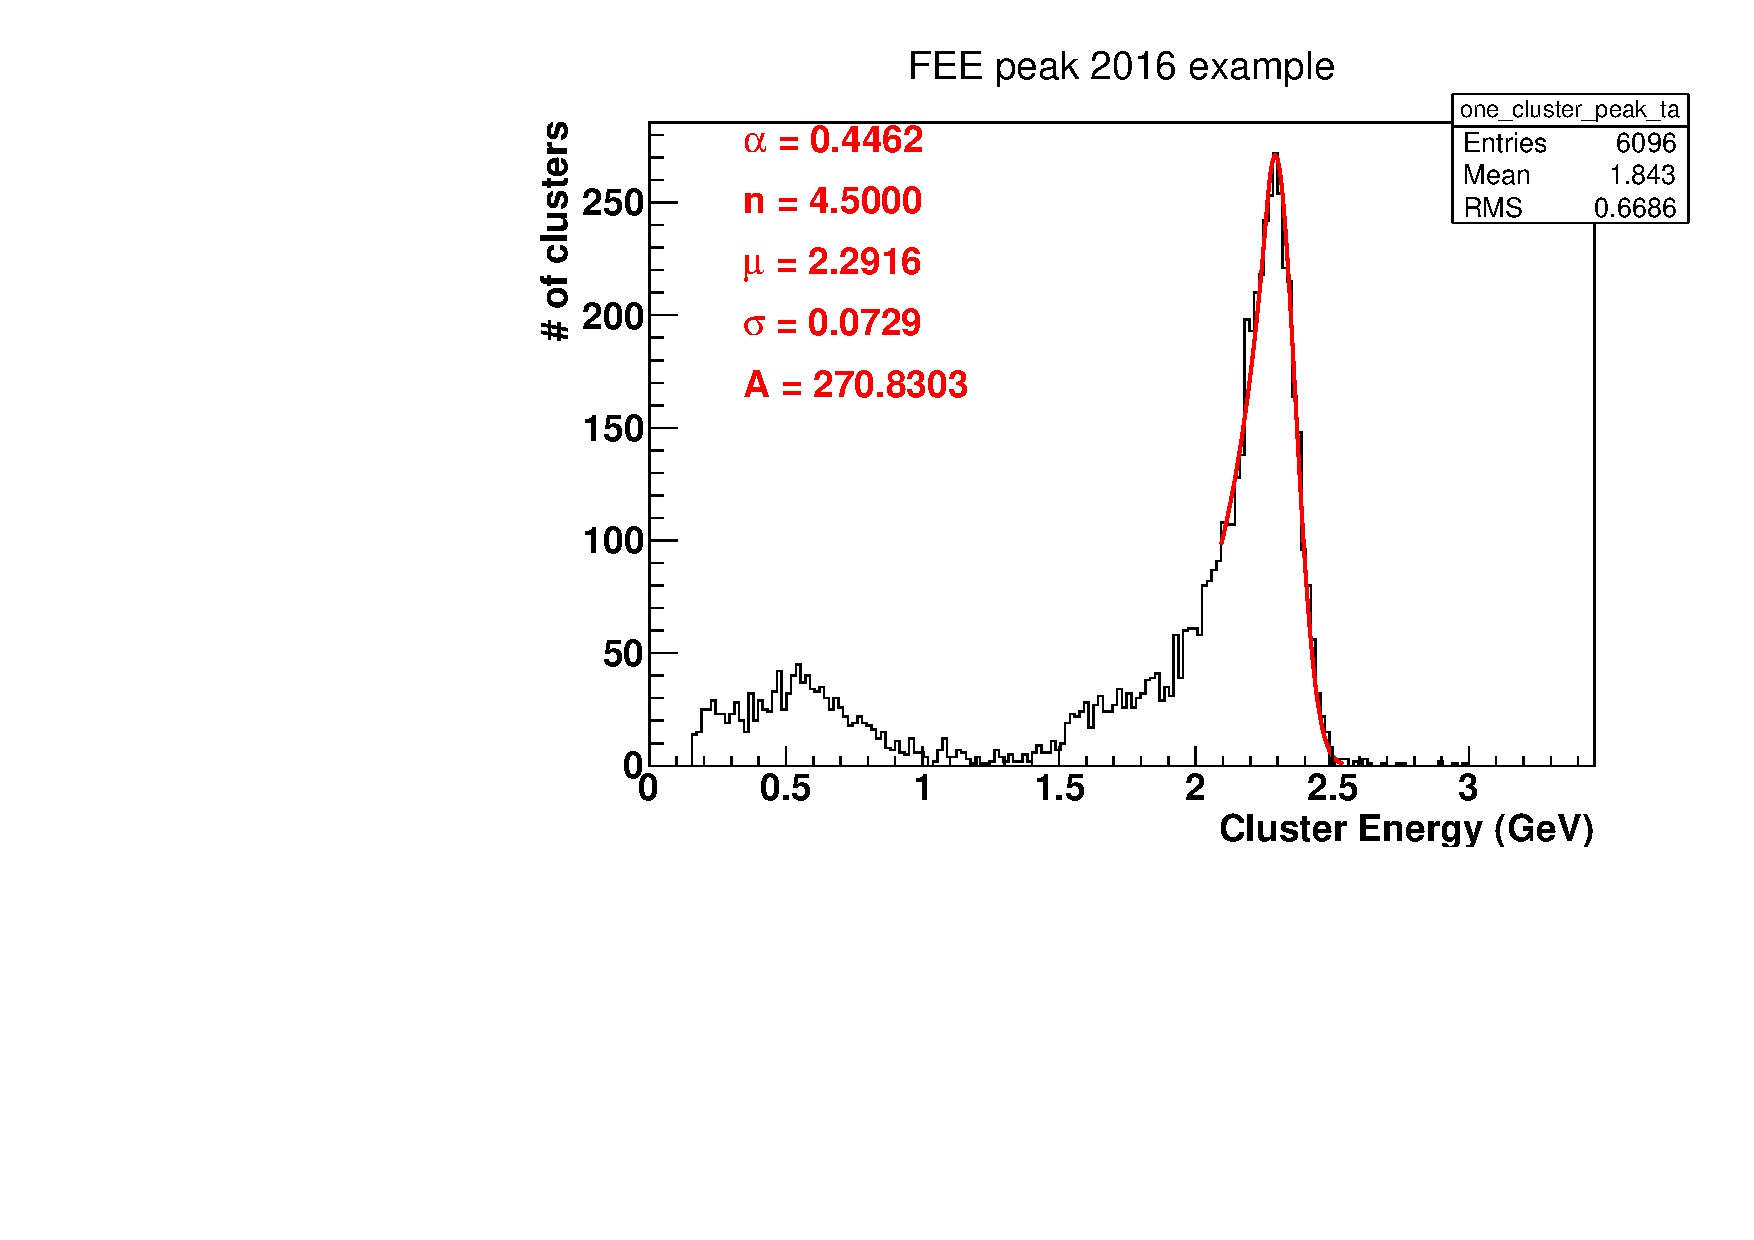
\includegraphics[width =  .9\textwidth]{figures/one2016_fit_example.pdf}
\caption{An example of a fit on the FEE peak in one of the runs in 2016.} 
\label{fig:one2016_fit_example}
\end{center}
\end{figure}

\begin{figure}[htbp] 
\begin{center}
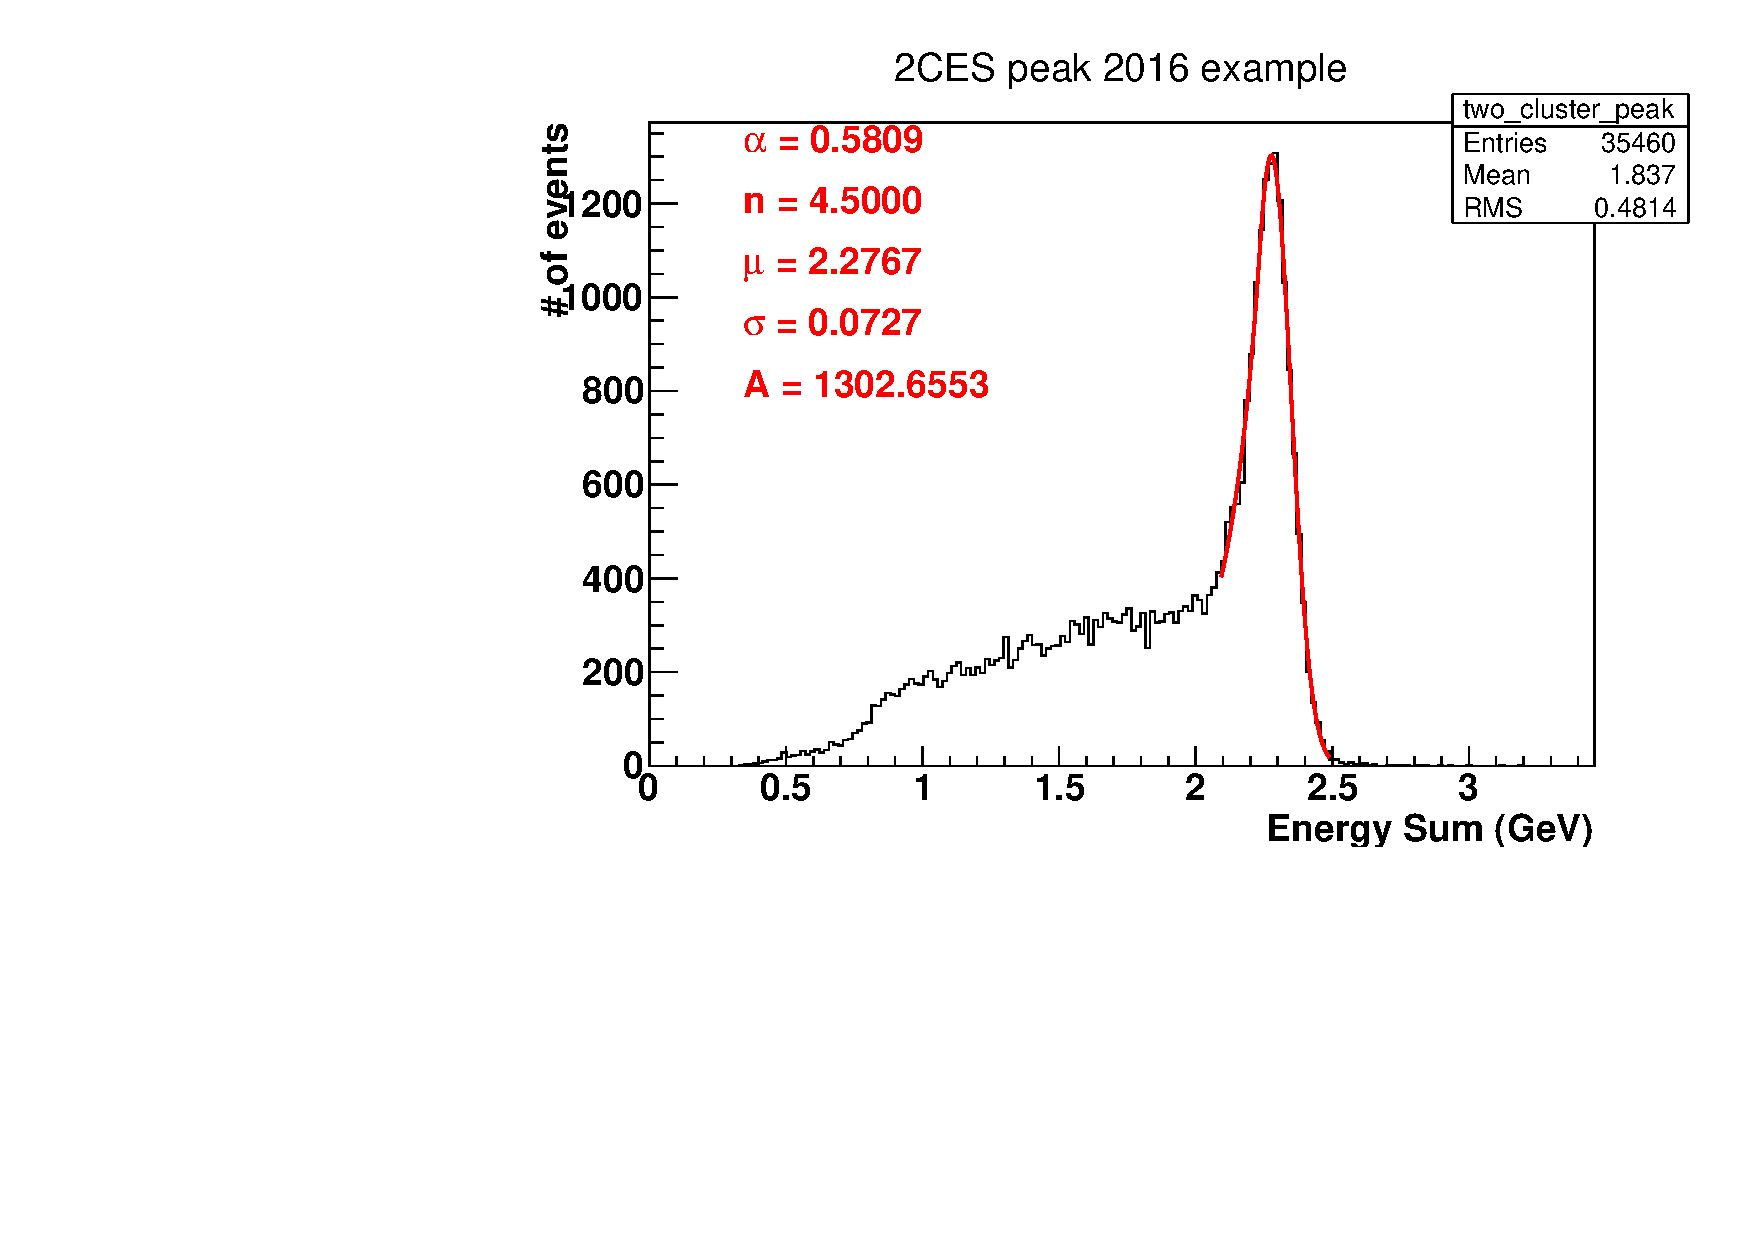
\includegraphics[width =  .9\textwidth]{figures/two2016_fit_example.pdf}
\caption{An example of a fit on the 2CES peak in one of the runs in 2016.} 
\label{fig:two2016_fit_example}
\end{center}
\end{figure}

\begin{figure}[htbp] 
\begin{center}
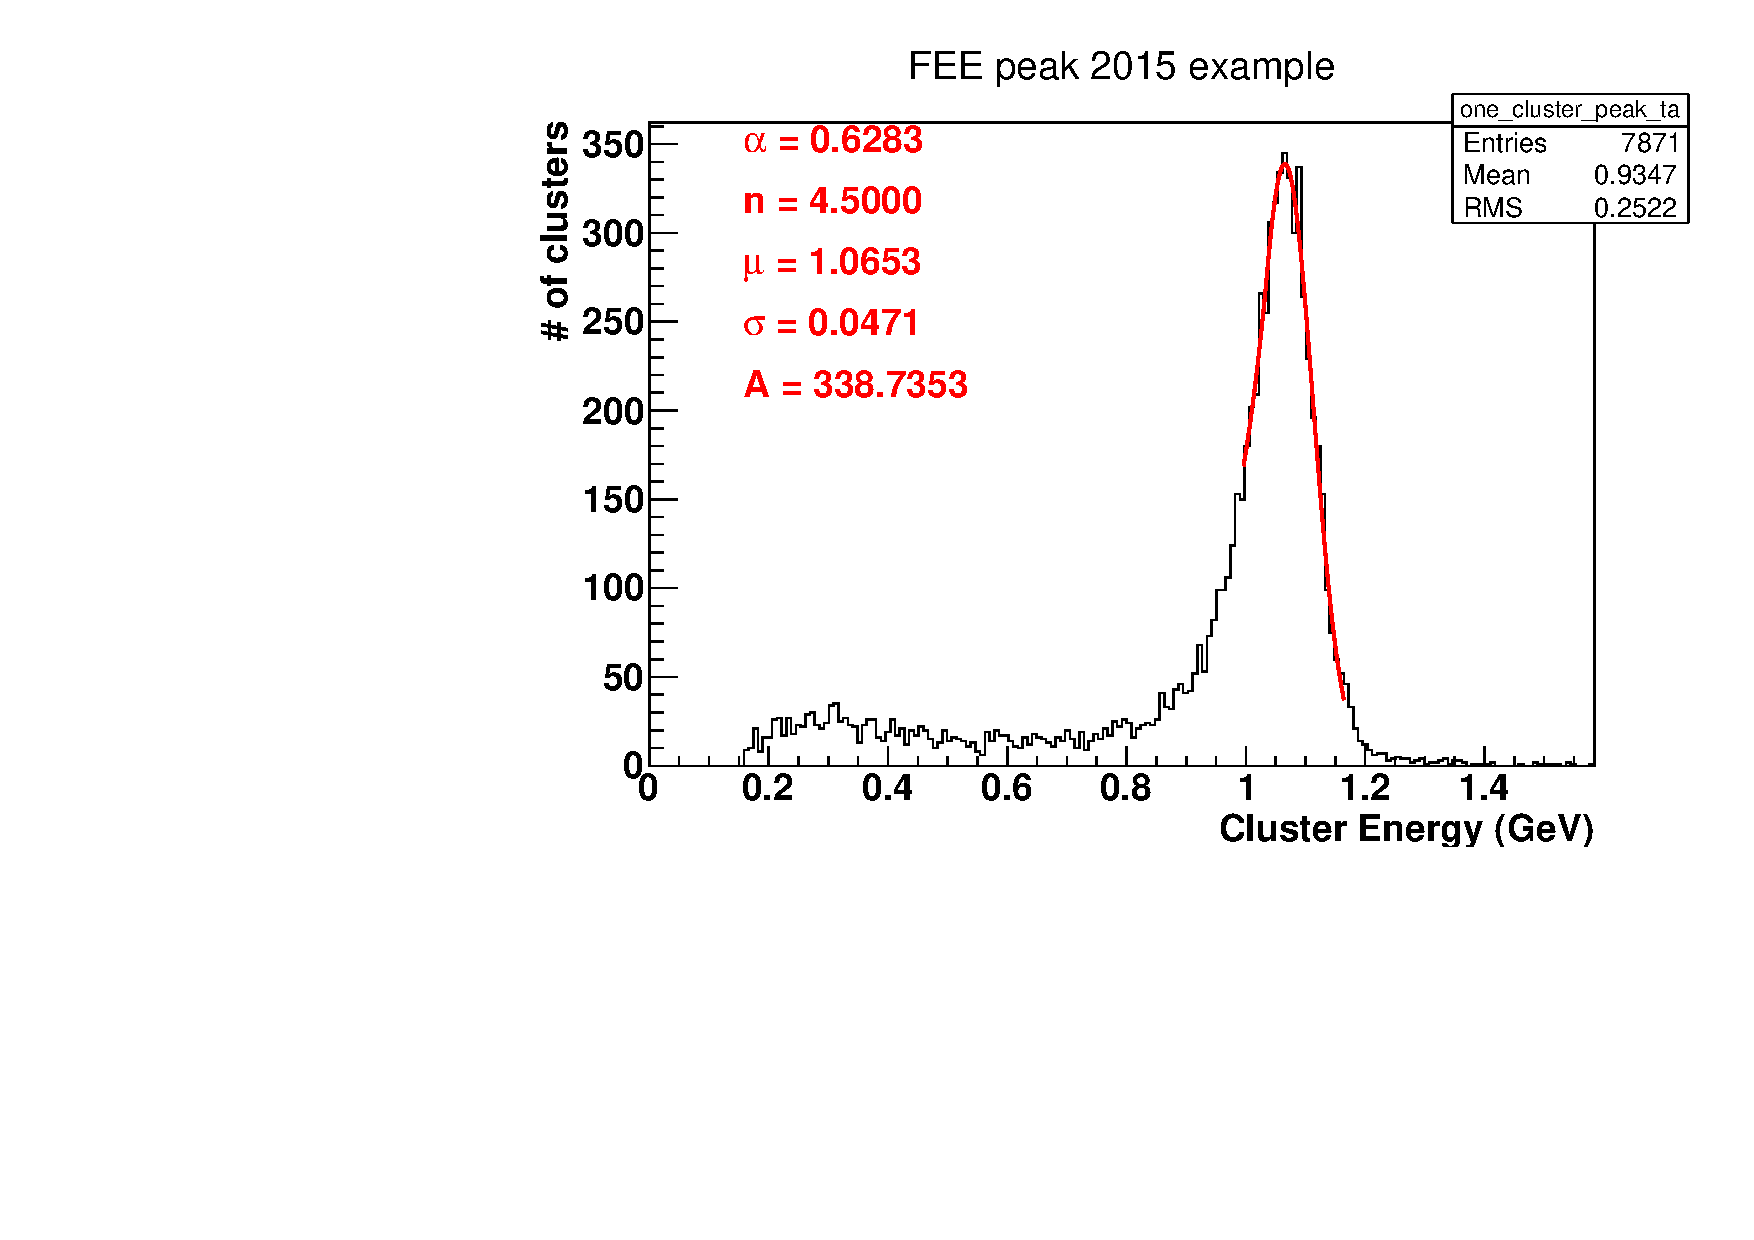
\includegraphics[width =  .9\textwidth]{figures/one2015_fit_example.pdf}
\caption{An example of a fit on the FEE peak in one of the runs in 2015.} 
\label{fig:one2015_fit_example}
\end{center}
\end{figure}

\begin{figure}[htbp] 
\begin{center}
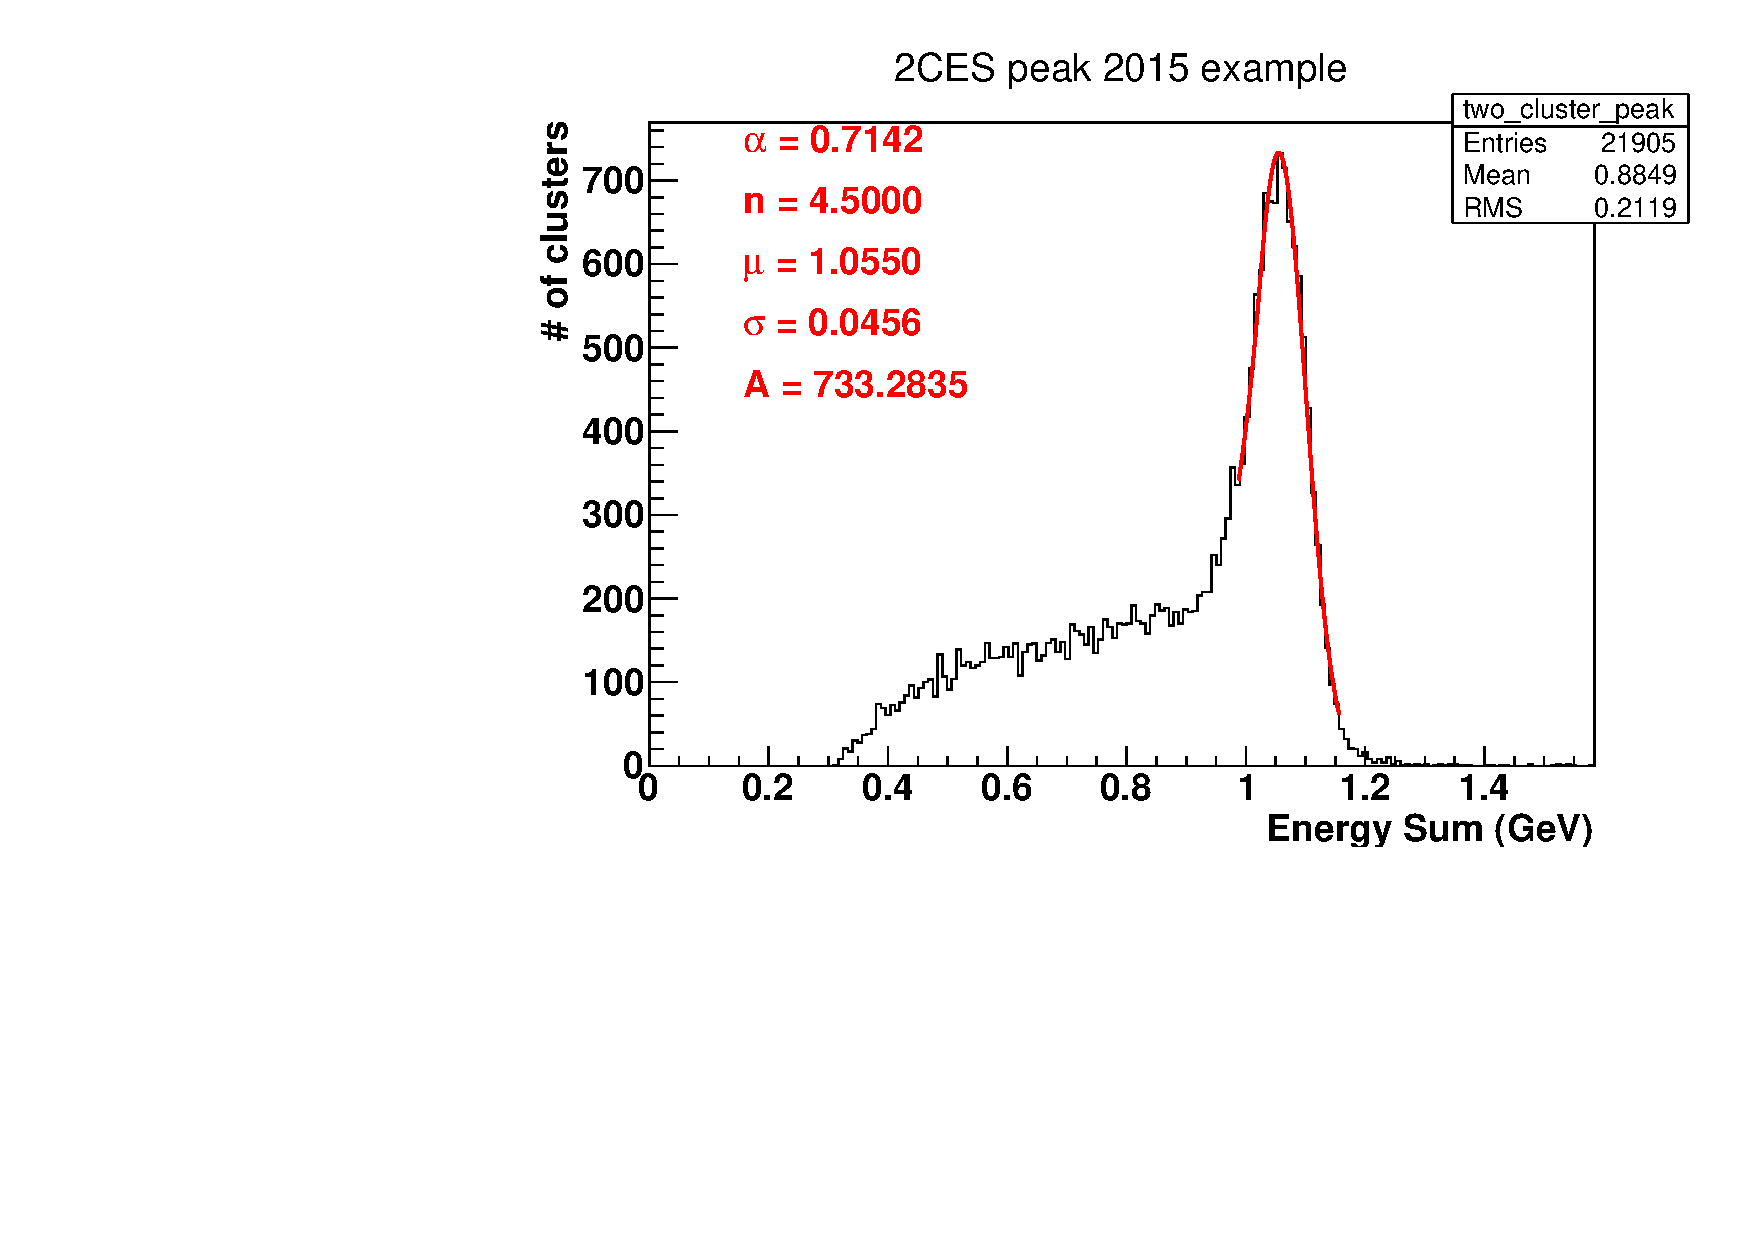
\includegraphics[width =  .9\textwidth]{figures/two2015_fit_example.pdf}
\caption{An example of a fit on the 2CES peak in one of the runs in 2015.} 
\label{fig:two2015_fit_example}
\end{center}
\end{figure}
\FloatBarrier
\section{Run Dependency}
In this section, I show the dependency of these peaks on the run number and on time in Figures \ref{fig:2016_run} through \ref{fig:2015_time}.  

\begin{figure}[htbp] 
\begin{center}
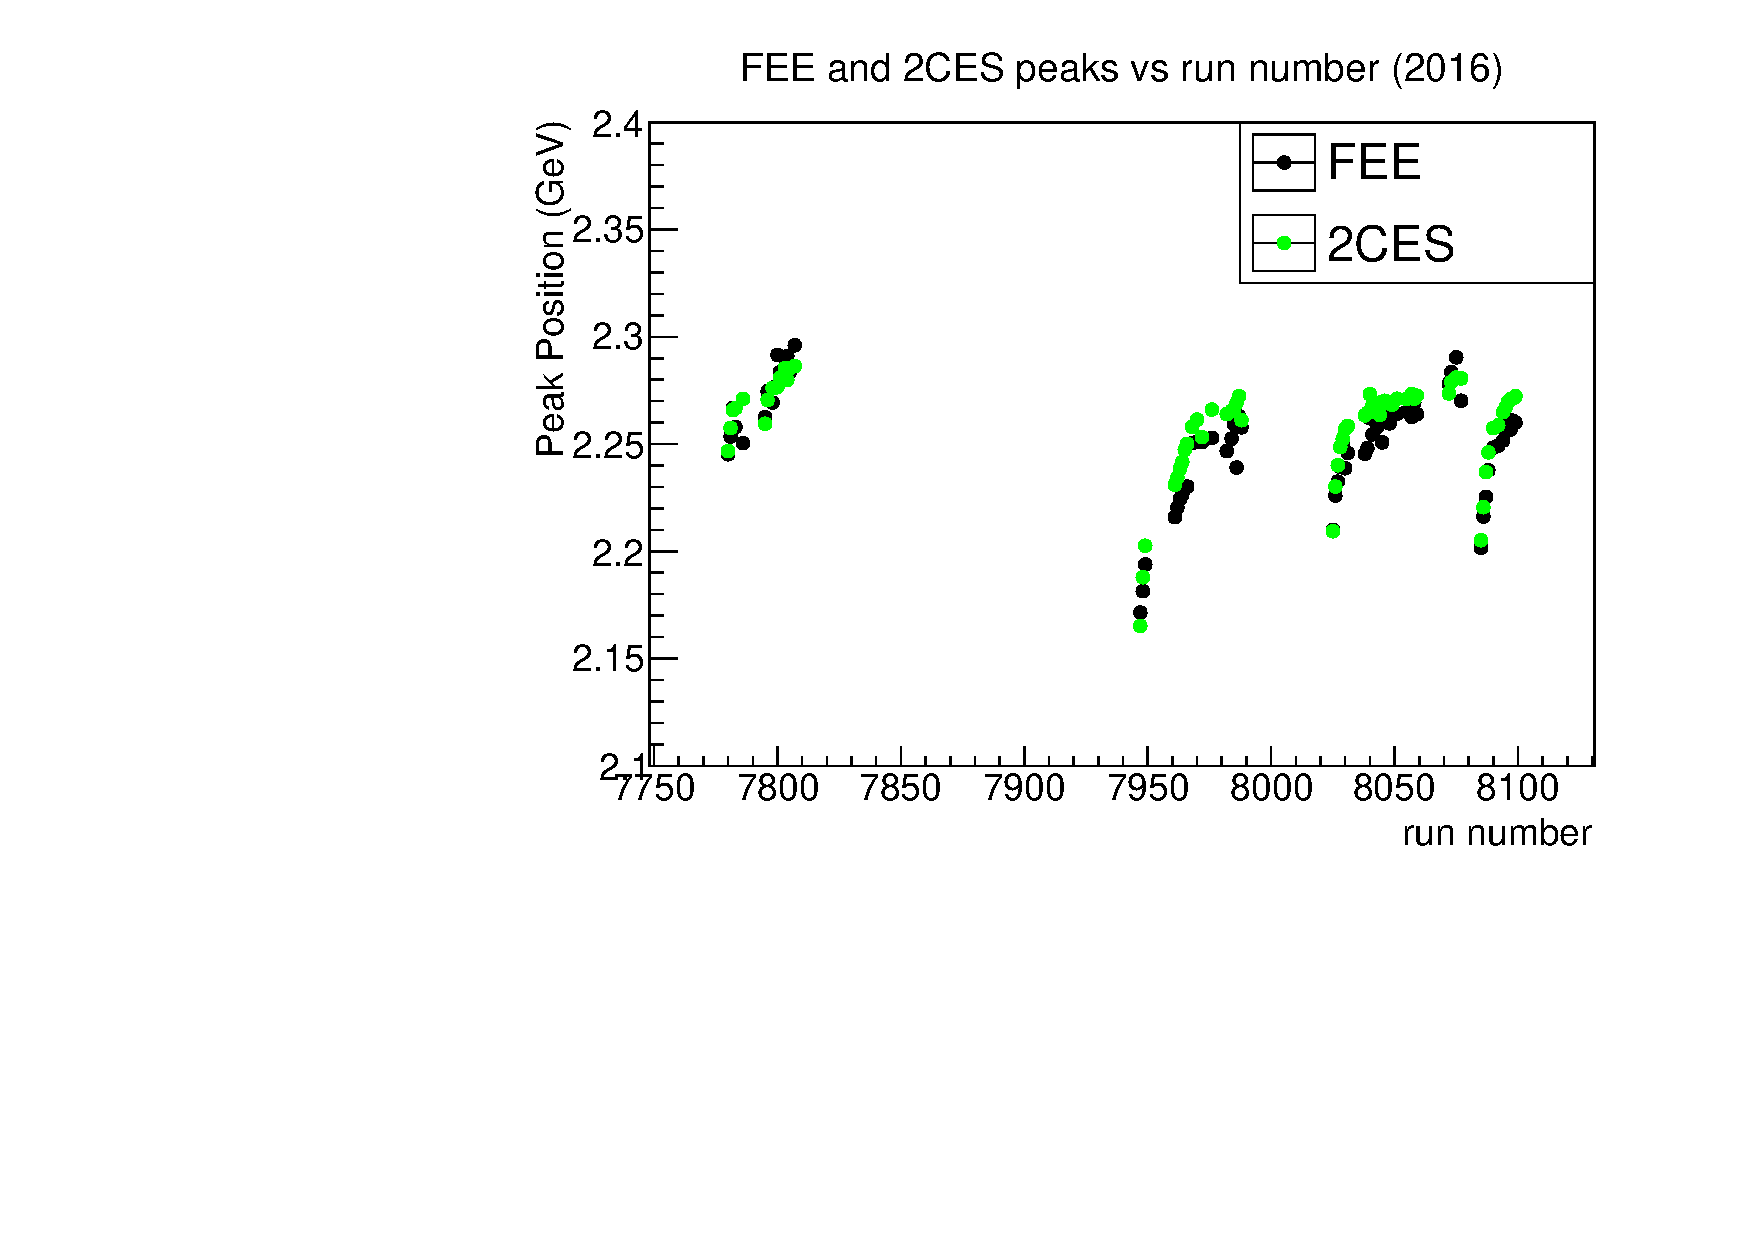
\includegraphics[width =  .9\textwidth]{figures/2016_run.pdf}
\caption{FEE (black) and 2CES (green) peak positions as a functions of run number in 2016.} 
\label{fig:2016_run}
\end{center}
\end{figure}

\begin{figure}[htbp] 
\begin{center}
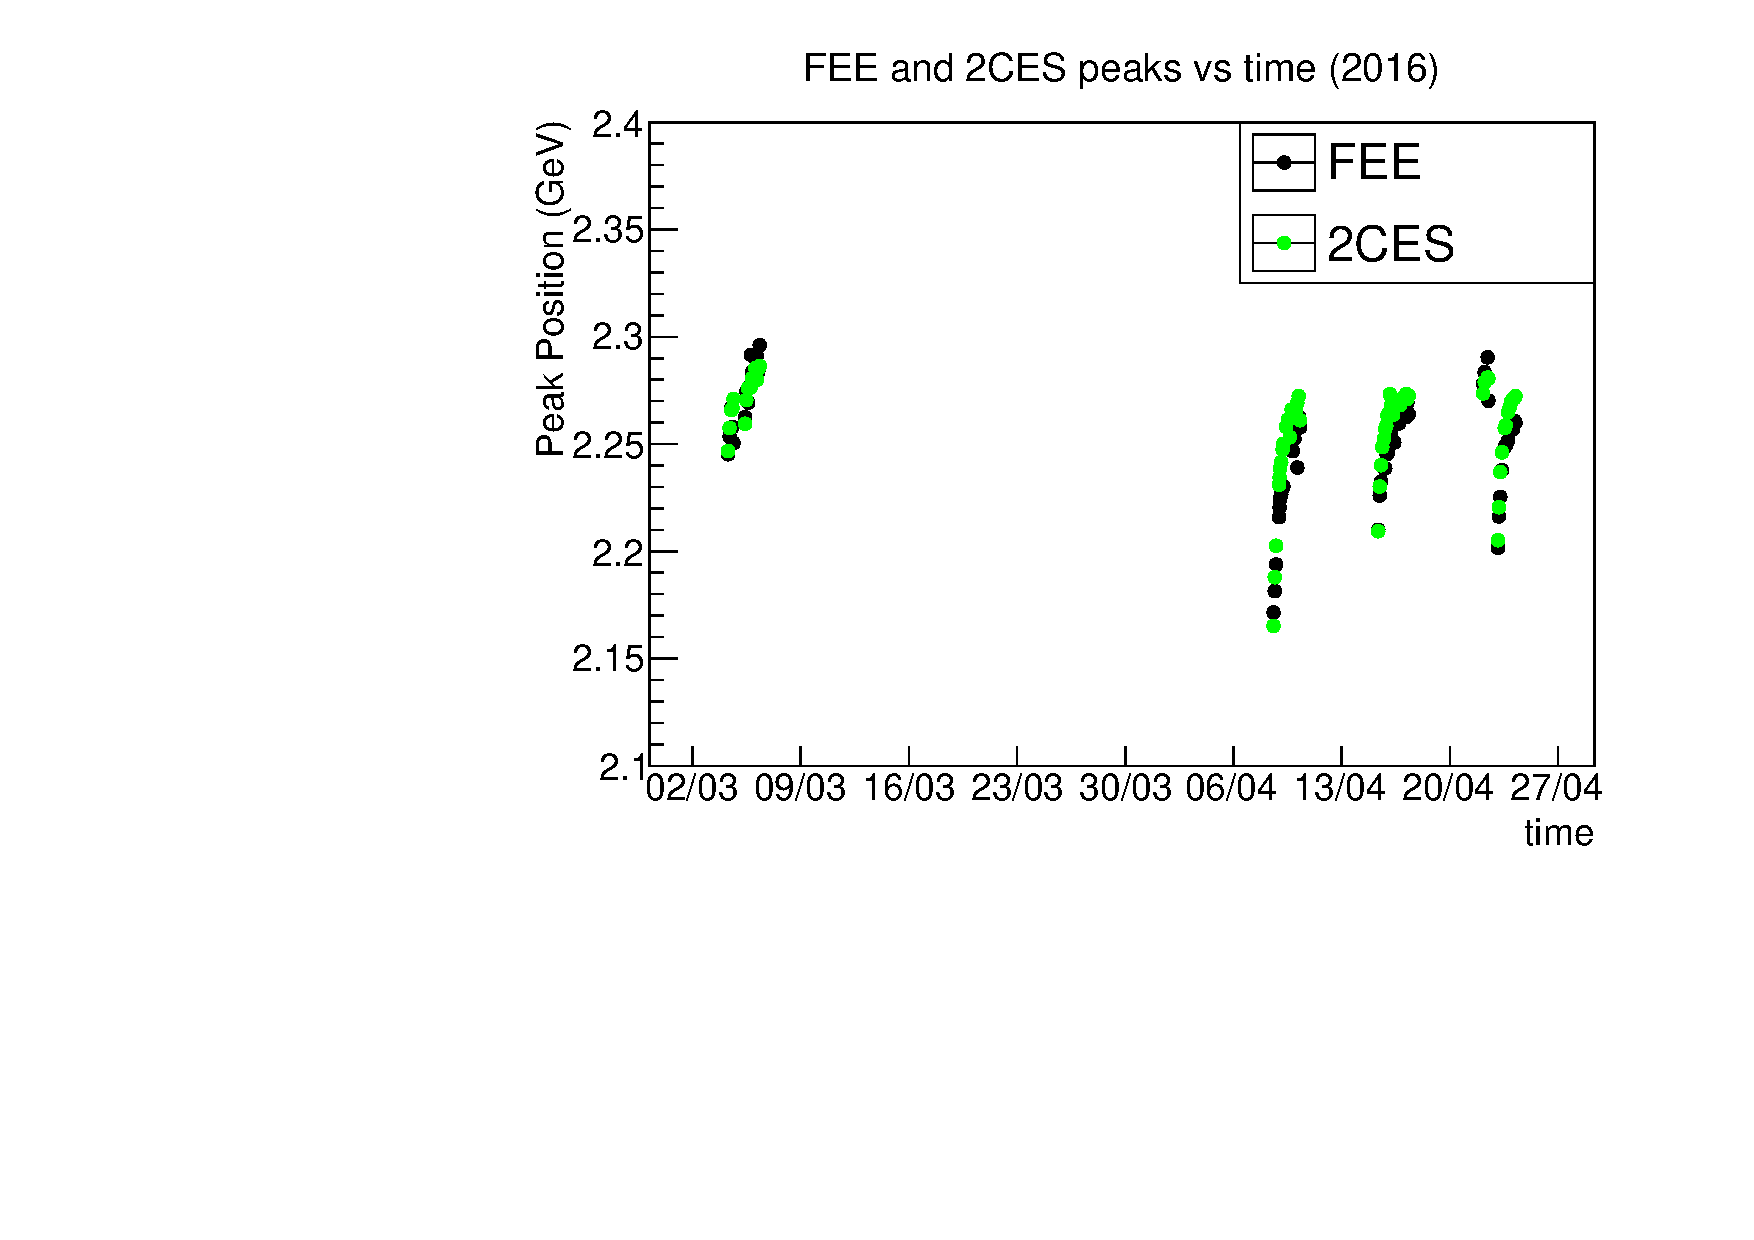
\includegraphics[width =  .9\textwidth]{figures/2016_time.pdf}
\caption{FEE (black) and 2CES (green) peak positions as a functions of time in 2016.} 
\label{fig:2016_time}
\end{center}
\end{figure}

\begin{figure}[htbp] 
\begin{center}
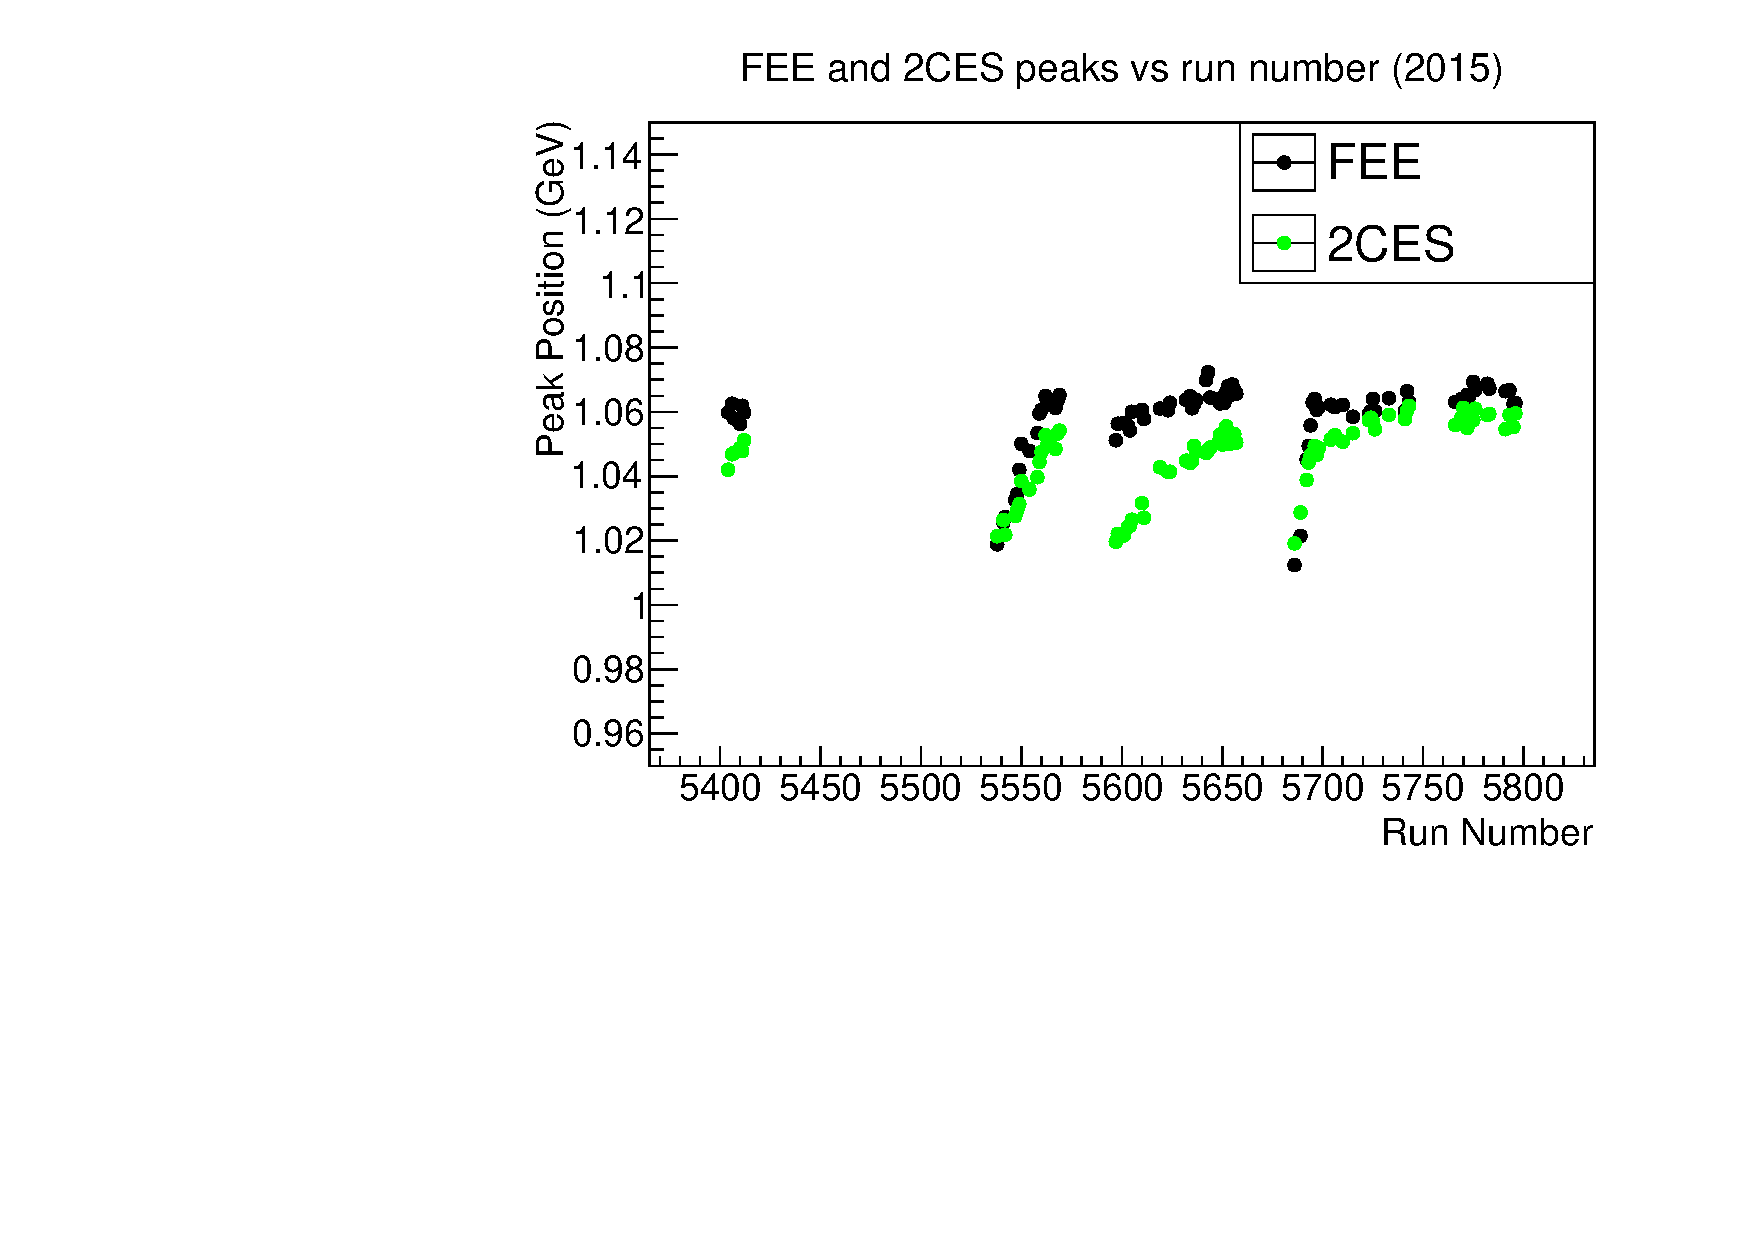
\includegraphics[width =  .9\textwidth]{figures/2015_run.pdf}
\caption{FEE (black) and 2CES (green) peak positions as a functions of run number in 2015.} 
\label{fig:2015_run}
\end{center}
\end{figure}

\begin{figure}[htbp] 
\begin{center}
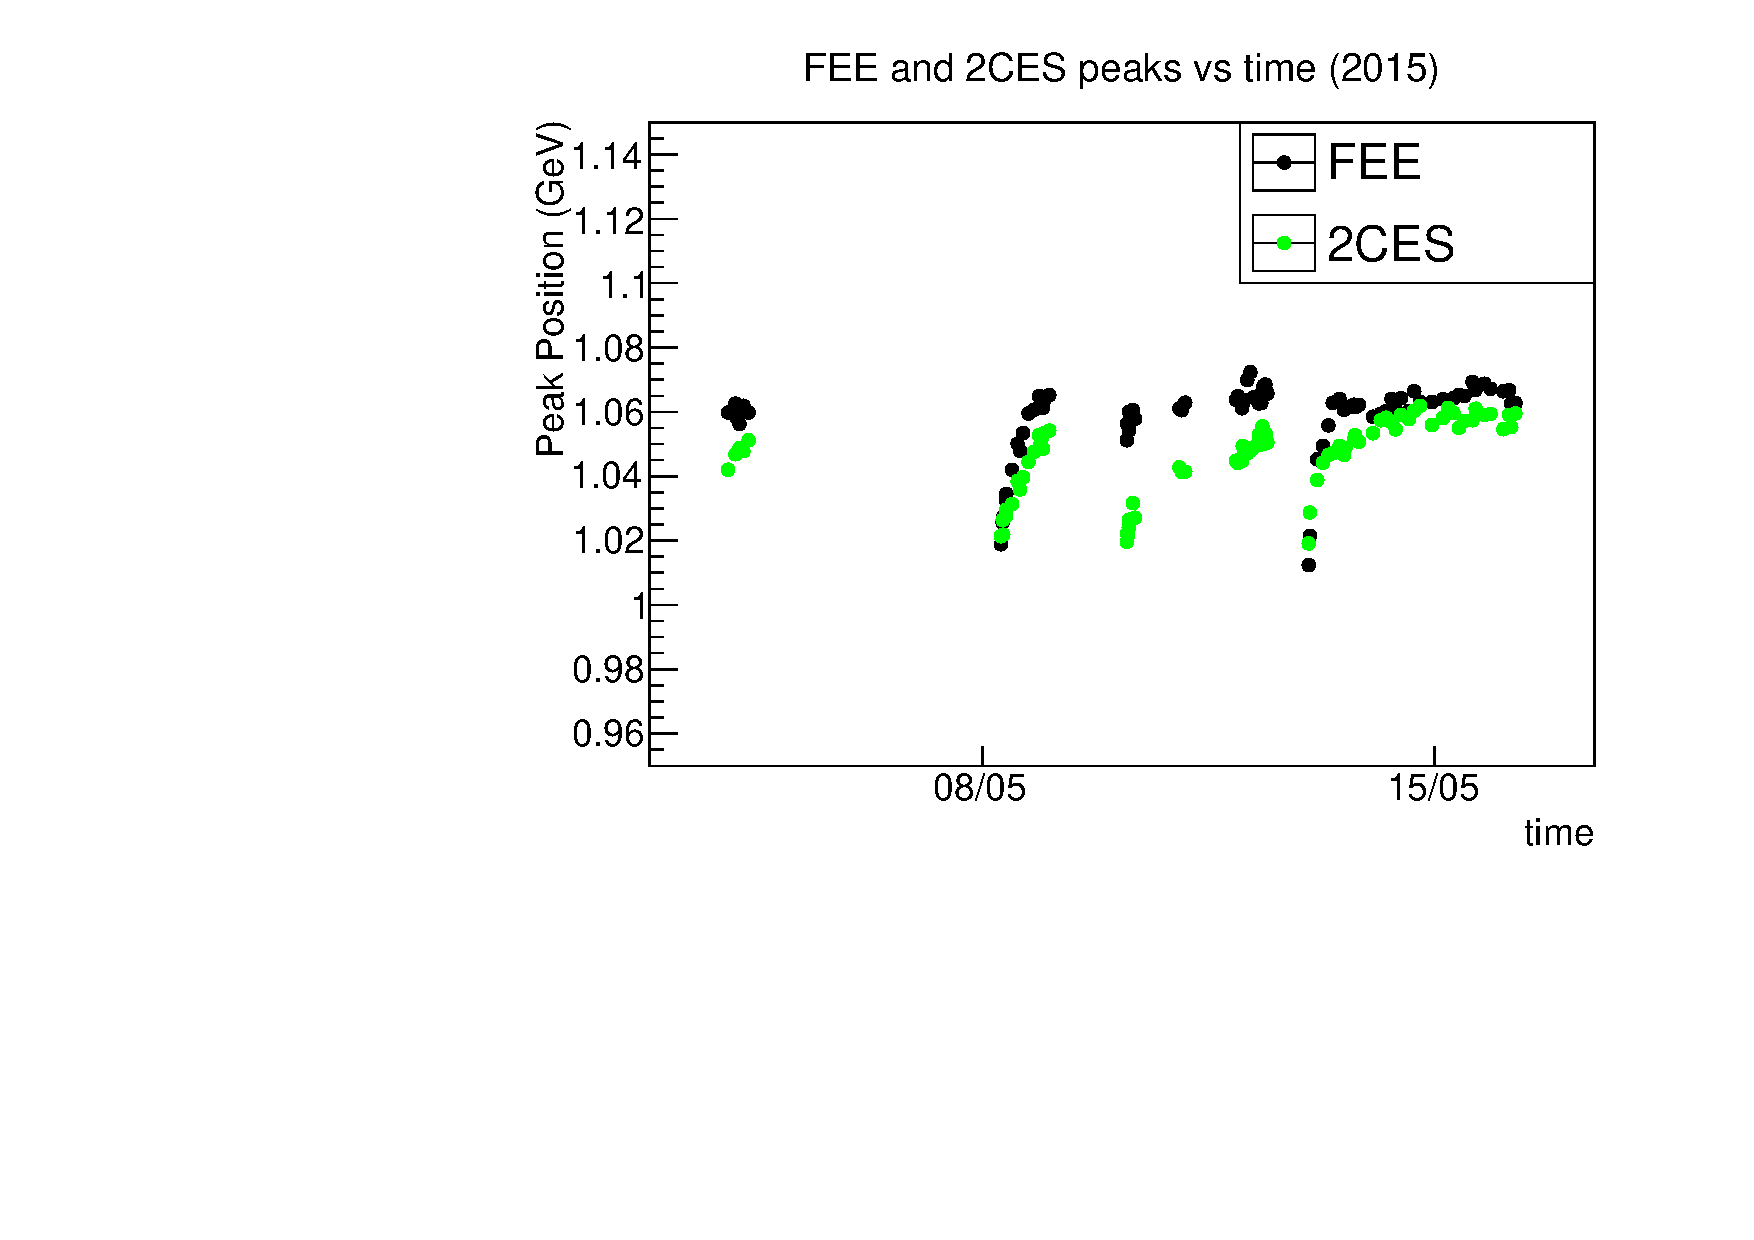
\includegraphics[width =  .9\textwidth]{figures/2015_time.pdf}
\caption{FEE (black) and 2CES (green) peak positions as a functions of time in 2015.} 
\label{fig:2015_time}
\end{center}
\end{figure}

\FloatBarrier
\section{Fitting the Run Dependency for the FEE peak}
I split both the 2015 and 2016 run periods into several segments (usually about a day or two in length) and fit the FEE peak position as a function of time using the following formula:

\begin{equation}
A - B \exp{-(t-t0)/C}
\label{eq:expo}
\end{equation}
 
where $A$, $B$ and $C$ are the fit parameters, and $t0$ is the timestamp at the beginning of the fit range, defined in terms of the seconds since the epoch in 1970 AD.  
 
In Figures \ref{fig:2016_time_fit} and
 \ref{fig:2015_time_fit} below I show these fits overlaid on the FEE peak positions graphs from Figures
  \ref{fig:2016_time} and
   \ref{fig:2015_time} above.  Table \ref{tab:time_fit} lists the parameters of the fits, and the time ranges for which they are applicable.



\begin{figure}[htbp] 
\begin{center}
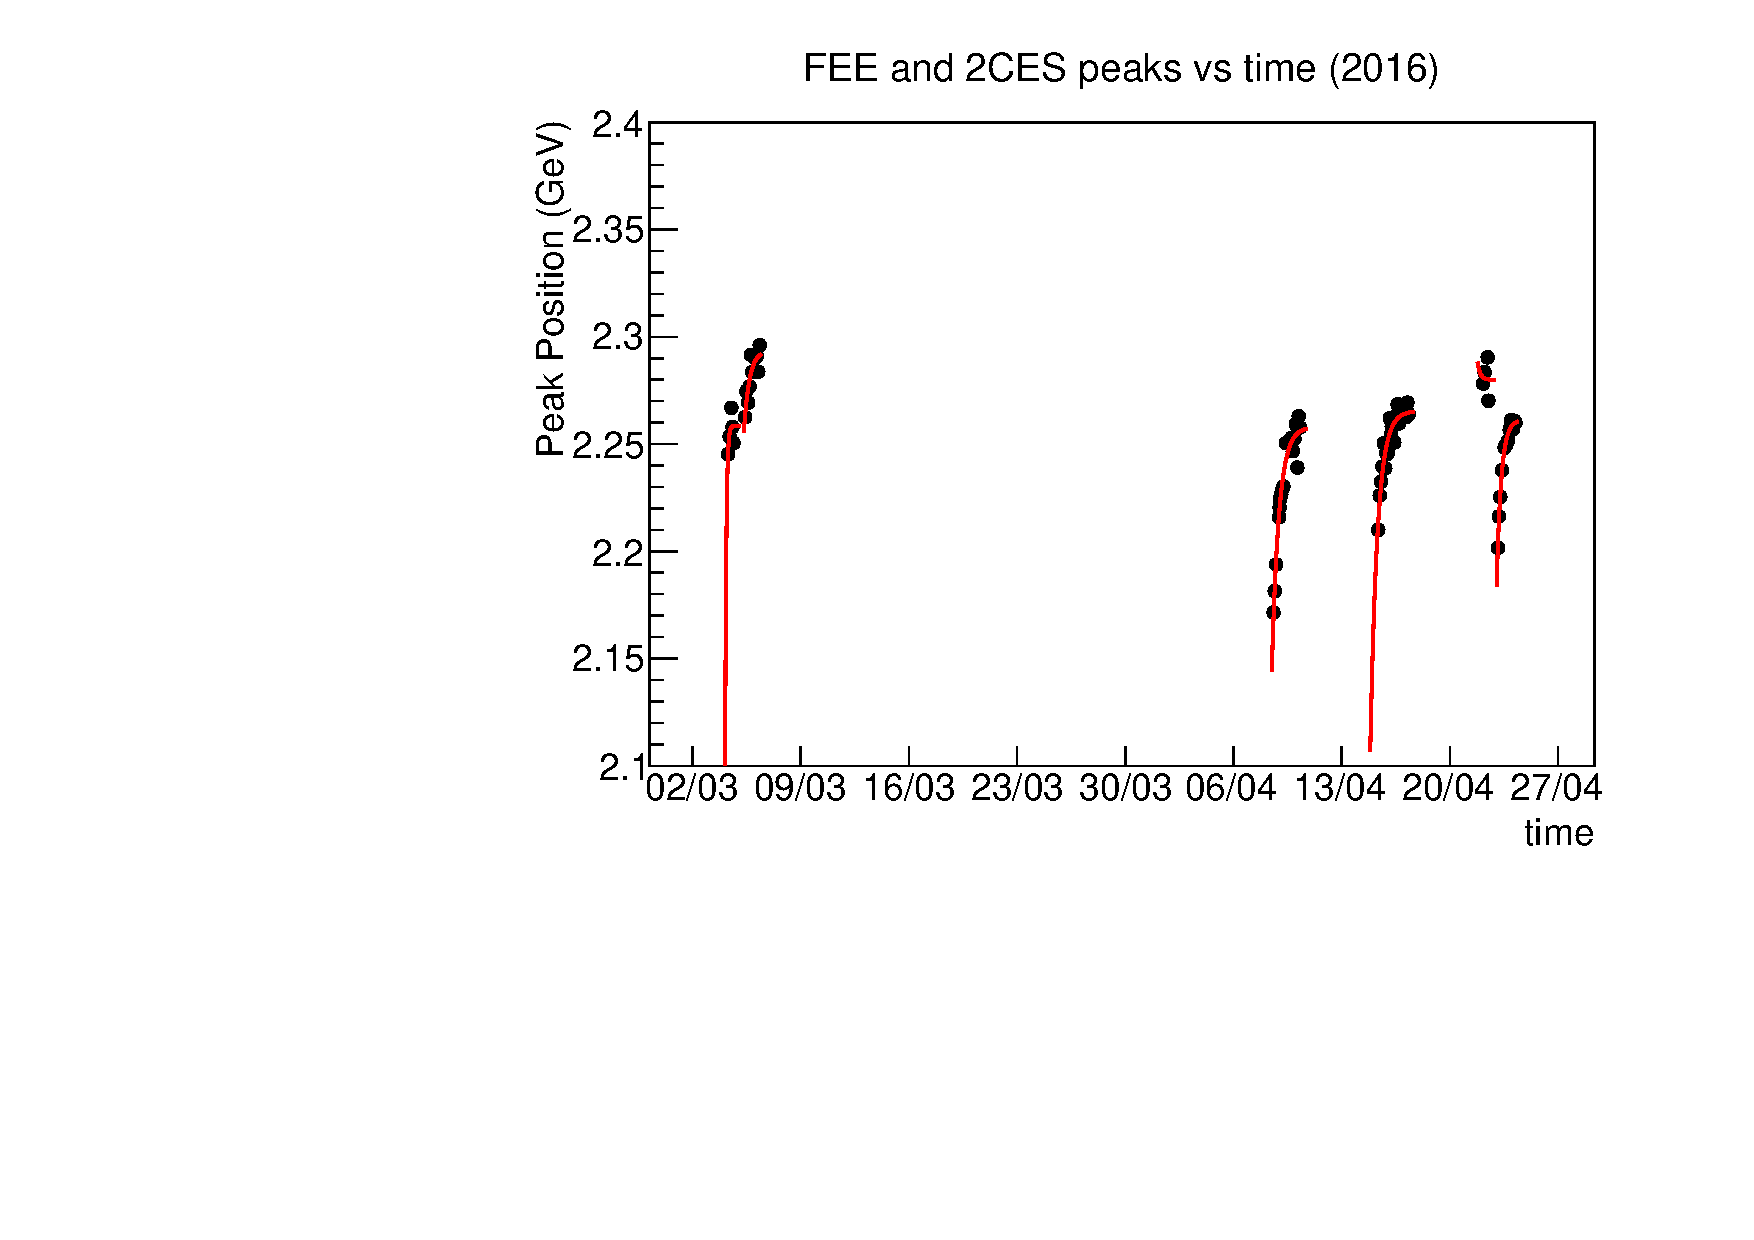
\includegraphics[width =  .9\textwidth]{figures/2016_time_fit.pdf}
\caption{Fit on the FEE peak position as a function of time in 2016.}
\label{fig:2016_time_fit} 
\end{center}
\end{figure}

\begin{figure}[htbp] 
\begin{center}
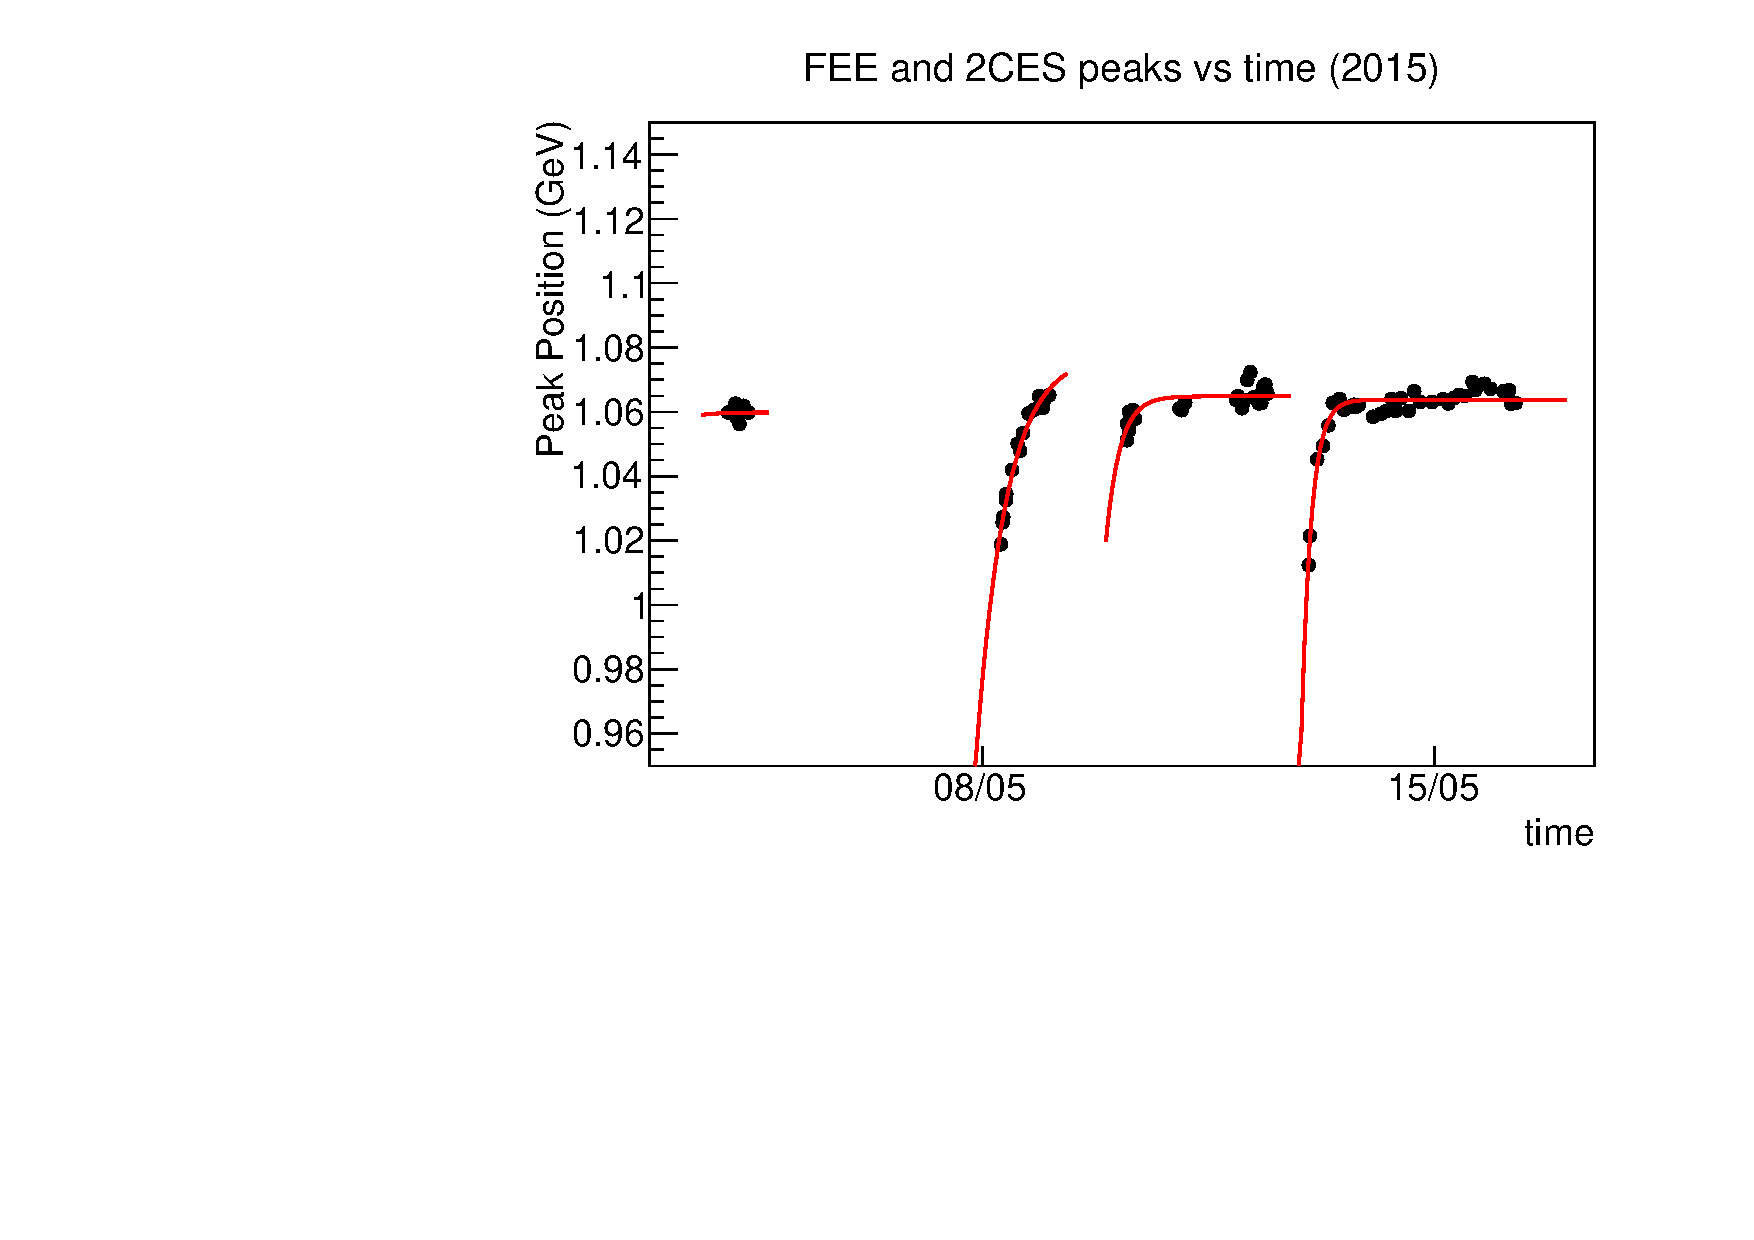
\includegraphics[width =  .9\textwidth]{figures/2015_time_fit.pdf}
\caption{Fit on the FEE peak position as a function of time in 2015.} 
\label{fig:2015_time_fit}
\end{center}
\end{figure}

\begin{table}[htp]
\caption{List of parameters of the fits to the FEE peak positions (both the 2015 and 2016 runs are included in this one table)}
\begin{center}
\begin{tabular}{|c|c|l|l|l|}
\hline
time start & time end & A (GeV) & B (GeV) & C (s) \\
\hline
1.43084e+09 & 1.43093e+09 & 1.05985 & 0.000777727 & 26833.2\\
1.4312e+09 & 1.43133e+09 & 1.07784 & 0.150727 & 39986.5\\
1.43138e+09 & 1.43163e+09 & 1.06485 & 0.048244 & 18662.8\\
1.43163e+09 & 1.432e+09 & 1.06381 & 0.276214 & 13123.3\\
\hline
1.45714e+09 & 1.45723e+09 & 2.2585 & 0.399416 & 6574.8\\
1.45725e+09 & 1.45735e+09 & 2.29357 & 0.0388658 & 30863.9\\
1.4602e+09 & 1.4604e+09 & 2.25799 & 0.117147 & 39662.9\\
1.46075e+09 & 1.461e+09 & 2.26538 & 0.163699 & 40000\\
1.46135e+09 & 1.46145e+09 & 2.27994 & -0.00861751 & 15844.2\\
1.46146e+09 & 1.46158e+09 & 2.26131 & 0.0794098 & 25784.6\\
\hline
\end{tabular}
\end{center}
\label{tab:time_fit}
\end{table}%


\FloatBarrier
\section{Corrected 2 Cluster Energy Sum:}

If my hypothesis that the cluster energies are uniformly scaled by a time dependent factor, then  the ratio of the 2 cluster energy sum to the FEE peak should be constant.  
To test this, I calculated the ``corrected" 2CES peak by multiplying the uncorrected 2CES peak by the beam energy divided by the parameterized value of the FEE peak.  Figures \ref{fig:twocorr2016} and 
\ref{fig:twocorr2015} show the ``corrected" values as a function of time.  

\begin{figure}[htbp] 
\begin{center}
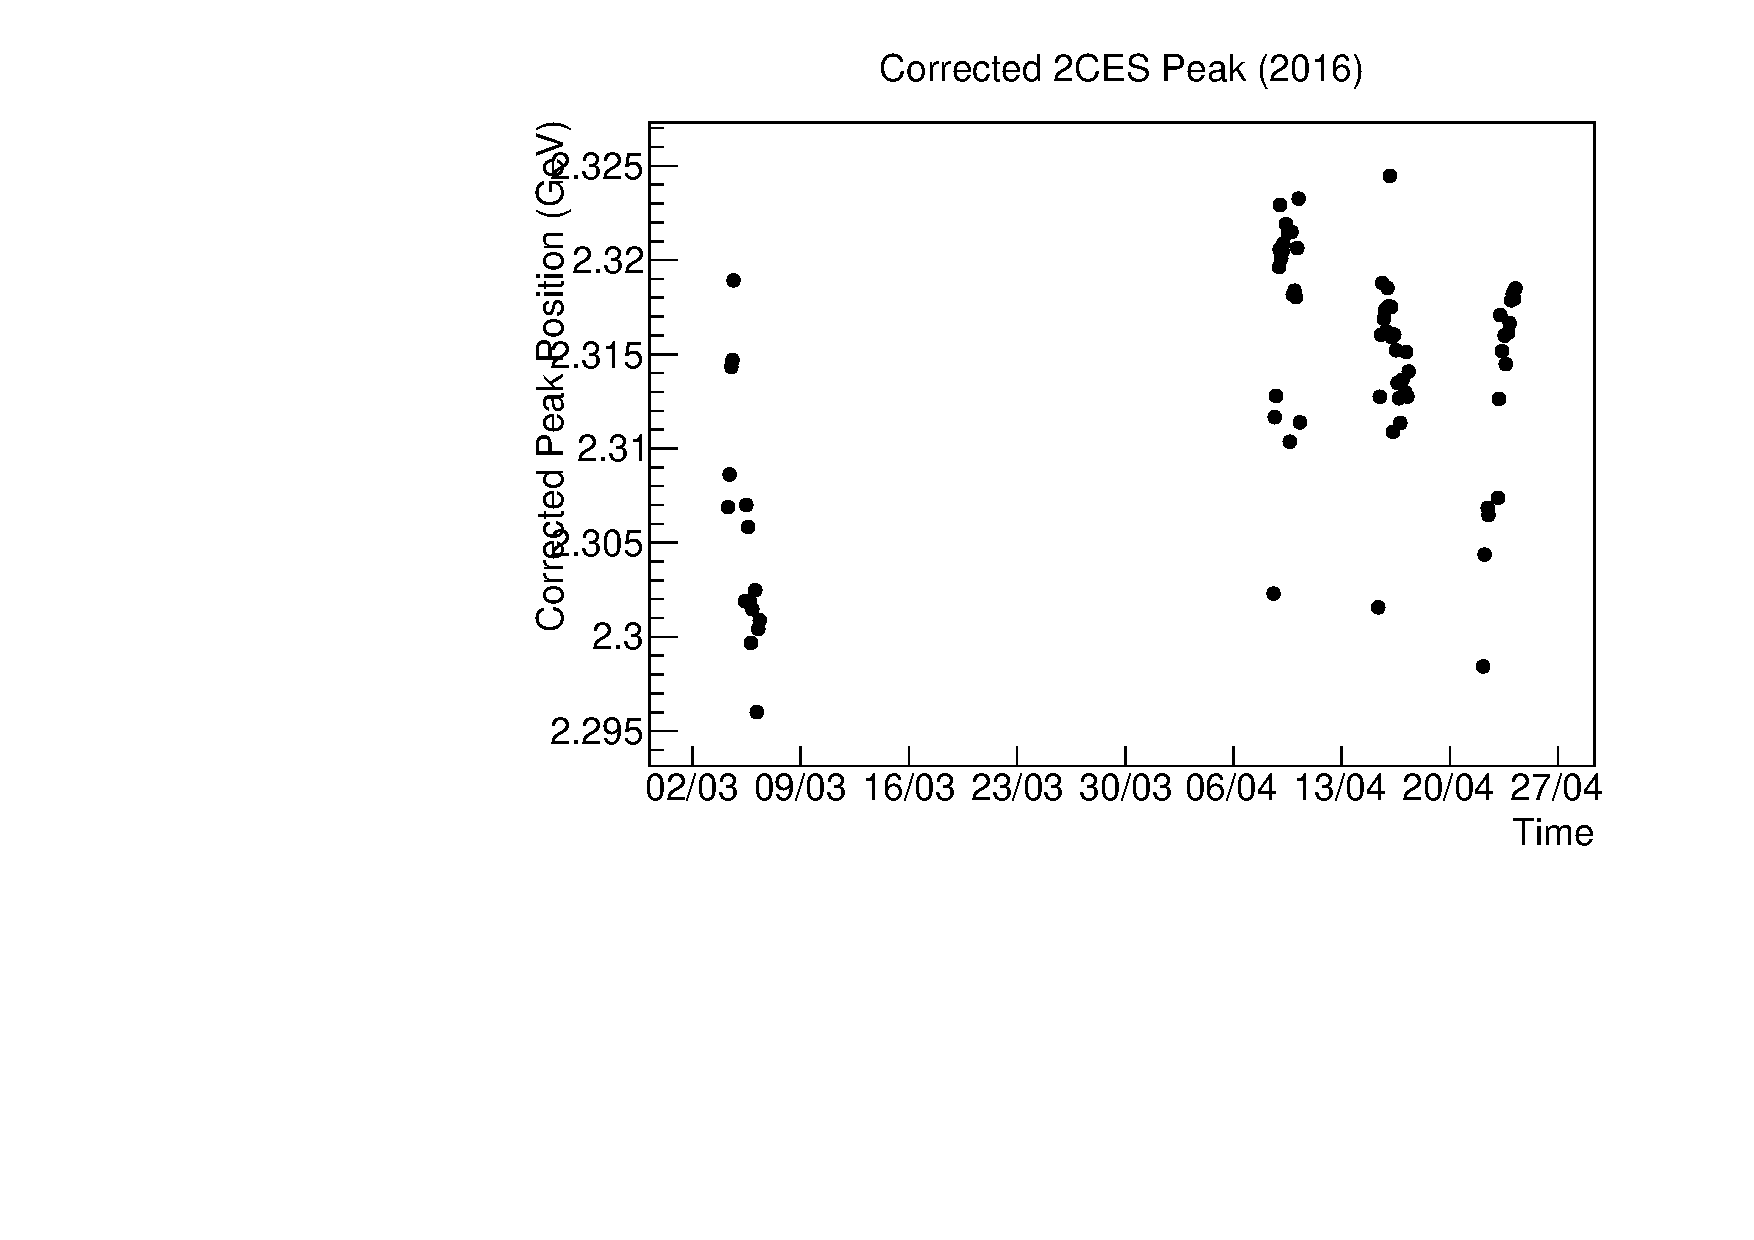
\includegraphics[width =  .9\textwidth]{figures/twocorr2016.pdf}
\caption{Corrected 2CES peak as a function of time in 2016.} 
\label{fig:twocorr2016}
\end{center}
\end{figure}

\begin{figure}[htbp] 
\begin{center}
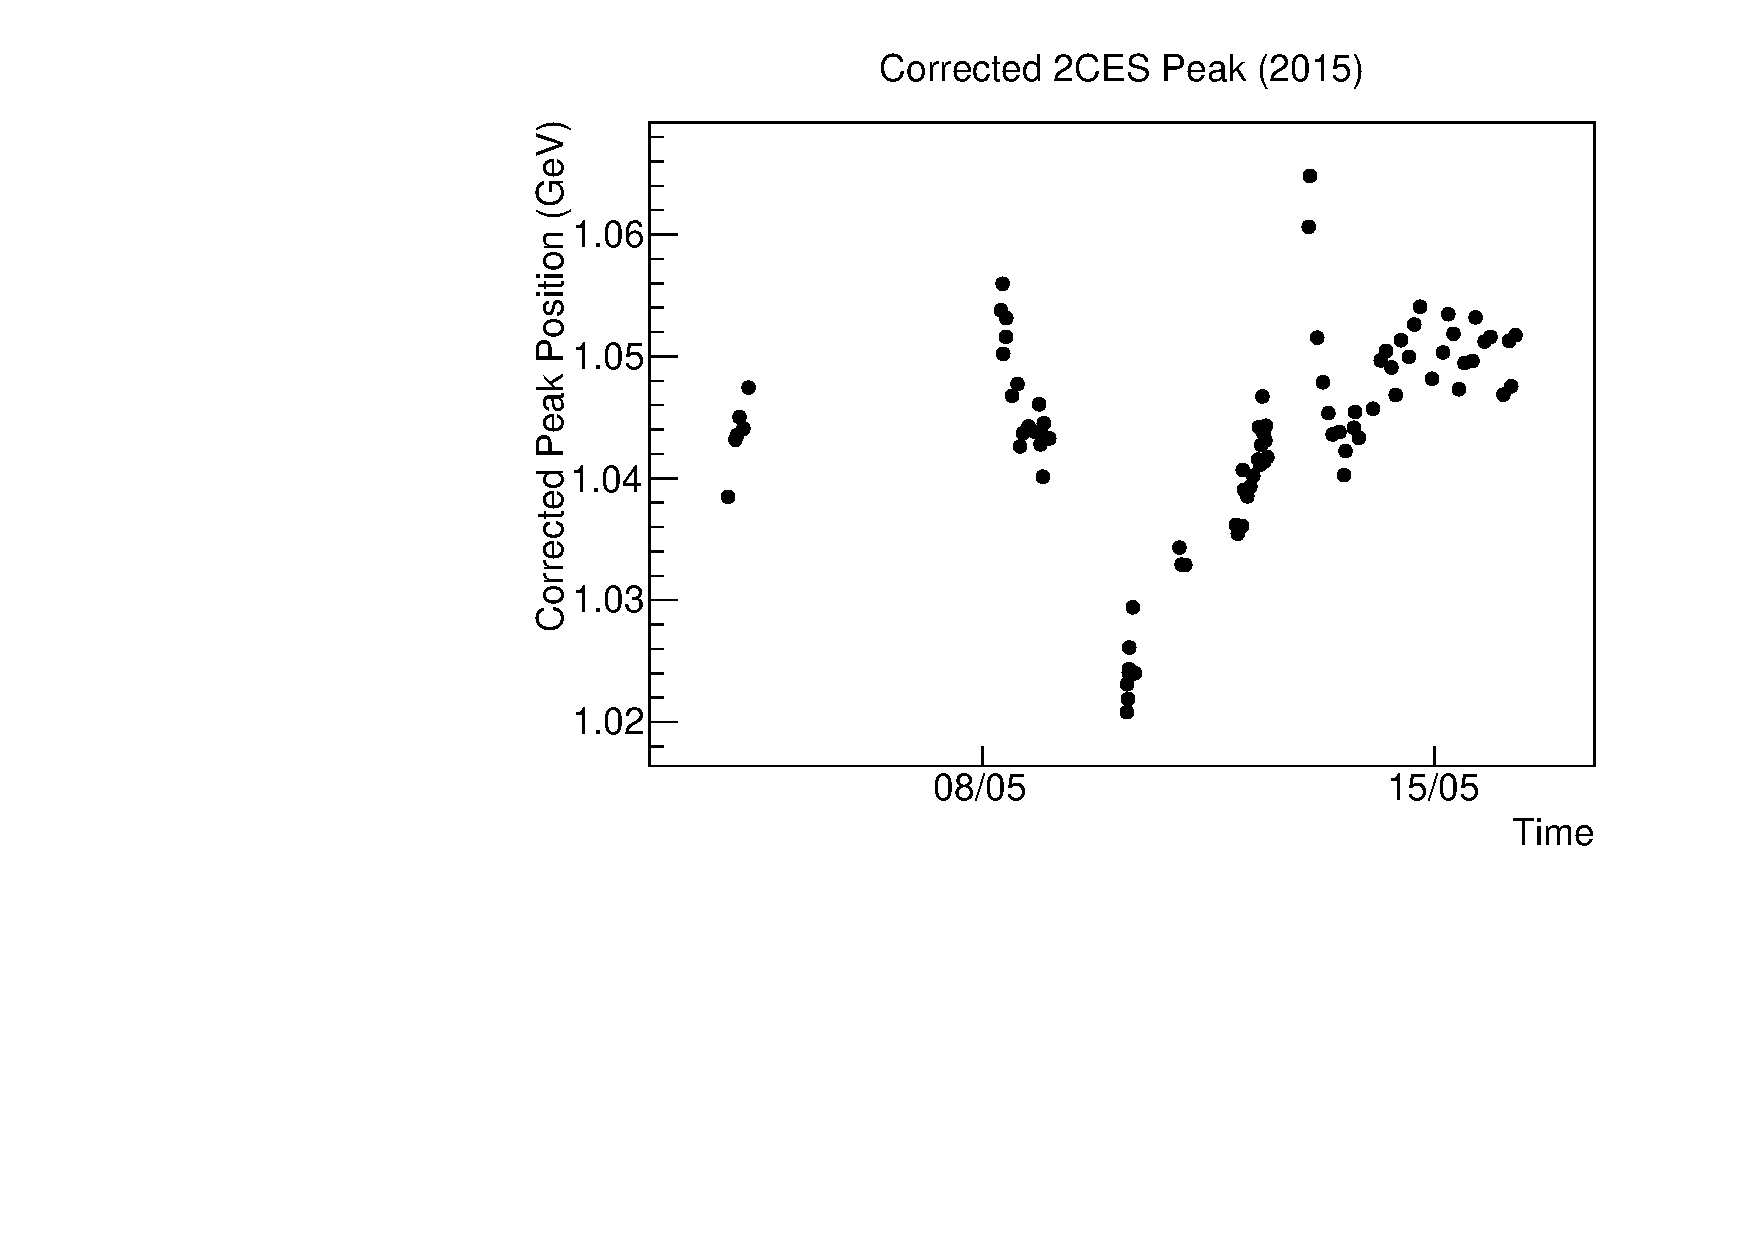
\includegraphics[width =  .9\textwidth]{figures/twocorr2015.pdf}
\caption{Corrected 2CES peak as a function of time in 2015.} 
\label{fig:twocorr2015}
\end{center}
\end{figure}
\FloatBarrier
\section{Conclusion}

Before the corrections, the mean value of the 2CES peak among the 2016 runs was 2.259 GeV with a standard deviation of 22.6 MeV.  After the corrections, the mean becomes 2.313 GeV and the standard deviation becomes 6.8 MeV.  For the 2015 dataset, the mean and standard deviation of the uncorrected 2CES peaks are 1.046 GeV and 8.4 MeV, and these become 1.044 GeV and 8.4 MeV after the corrections.  

In my opinion, the time dependent corrections are sufficient for the 2016 dataset, but they seem to make things worse in the 2015 dataset.  In \ref{{fig:2015_run}, it is already clear that the ratio of the 2CES peak to the FEE peak varies in an inconsistent manner.  This requires further investigation to determine the cause of this discrepency.  



\end{document}